\documentclass[10pt]{beamer}
\usepackage[T1]{fontenc}
\usepackage[latin1]{inputenc}
\usepackage[english]{babel}
\usepackage{setspace}
\usepackage{hyperref}


\title{DevOps - Modern Software Development}
\author{Oliver Zott}
\date{2024-05-08}


\begin{document}
\setstretch{1.5} % Set line spacing to 1.5 (adjust as needed)

% --------------------------------------------------------------------------------------------------------------------------
\begin{frame}
	\titlepage
	\vfill
    \centering
    \href{https://github.com/OliverZott/python-devops-example}{GitHub Repository}
\end{frame}

% --------------------------------------------------------------------------------------------------------------------------
\begin{frame}{Table of Contents}
 	\tableofcontents
\end{frame}

% =============================================================
\section{Survey}
% Quick survey to establish common ground

\begin{frame}{Survey}
	\begin{itemize}
		\item Scrum / Colaboration Tools (Github Project, Azure DevOps, Jira, Trello, etc.)
	\end{itemize}
\end{frame}

\begin{frame}{Survey}
	\begin{itemize}
		\item Scrum / colaboration tools (Github Project, Azure DevOps, Jira, Trello, etc.)
		\item Git / PullRequest / Code Review
	\end{itemize}
\end{frame}

\begin{frame}{Survey}
	\begin{itemize}
		\item Scrum / colaboration tools (Github Project, Azure DevOps, Jira, Trello, ...)
		\item Git / PullRequest / Code Review
		\item Linting/Analyze-Tools (Ruff, SonarQube, ...)
	\end{itemize}
\end{frame}

\begin{frame}{Survey}
	\begin{itemize}
		\item Scrum / colaboration tools (Github Project, Azure DevOps, Jira, Trello, etc.)
		\item Git / PullRequest / Code Review
		\item Linting/Analyze-Tools (Ruff, SonarQube, ...)
		\item Testing (pipeline, pre-commit hooks, QA, ...)
	\end{itemize}
\end{frame}

\begin{frame}{Survey}
	\begin{itemize}
		\item Scrum / colaboration tools (Github Project, Azure DevOps, Jira, Trello, etc.)
		\item Git / PullRequest / Code Review
		\item Linting/Analyze-Tools (Ruff, SonarQube, ...)
		\item Testing (pipeline, pre-commit hooks, QA, ...)
		\item CI / CD pipelines
	\end{itemize}
\end{frame}


% =============================================================
\section{Introduction to DevOps}
\begin{frame}{DevOps}
    \begin{center}
        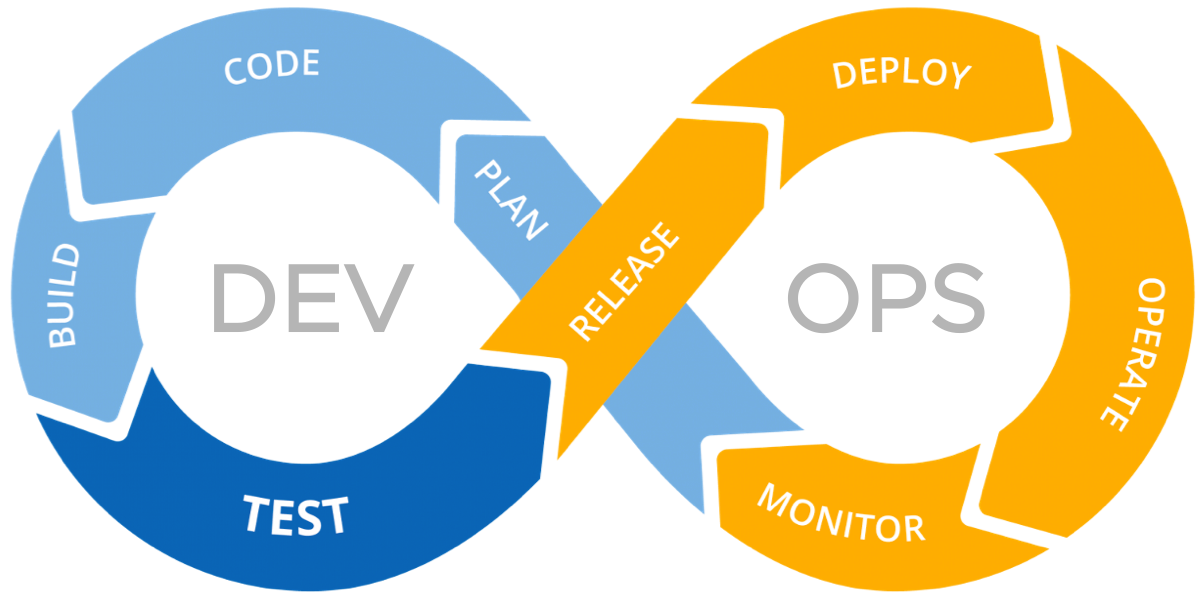
\includegraphics[width=9cm]{devops_lifecycle.png}
        \begin{figure}
            \caption{DevOps Lifecycle (\url{http://blogs.vmware.com/management/files/2020/03/2020-03-02_14-18-57.png} 2024-05-02)}
        \end{figure}
    \end{center}
\end{frame}

% --------------------------------------------------------------------------------------------------------------------------

\begin{frame}{DevOps}
	\begin{center}
		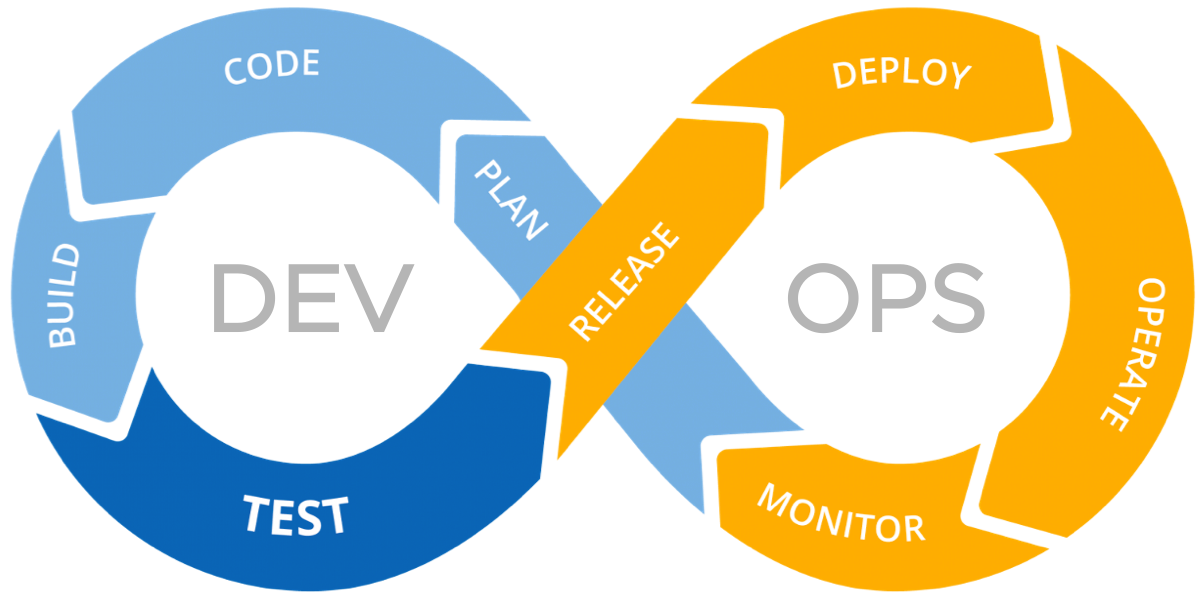
\includegraphics[width=4cm]{devops_lifecycle.png}
			\begin{figure}
				\caption{DevOps Lifecycle (\url{http://blogs.vmware.com/management/files/2020/03/2020-03-02_14-18-57.png} 2024-05-02)}
			\end{figure}
	\end{center}

	\begin{itemize}
		\item Plan/Collaborate
		\item Coding
		\item CI/CD
		\item Operate and Monitor (Containerization)
	\end{itemize}
\end{frame}


% =============================================================
\section{Example - PyPI}
\begin{frame}{Example - PyPI}
	Sample python package with a bug that needs fixing (\href{https://github.com/OliverZott/python-devops-example}{\color{blue}GitHub}, \href{https://pypi.org/project/velosaurus-calc/}{\color{blue}PyPI}).

	\begin{itemize}
		\item Planning with estimation
		\item Coding with AI support (including unit test)
		\item Check pipelines
	\end{itemize}
\end{frame}


% =============================================================
\section{Example - Docker}
\begin{frame}{Example - Docker Container}
	Sample asp.net core web API project with Docker containerization and Docker Hub deployment (\href{https://github.com/OliverZott/velosaurus-backend}{\color{blue}GitHub}, \href{https://hub.docker.com/repository/docker/dasmuesli/velosaurus-backend}{\color{blue}Docker Hub}).
	
	

	\begin{itemize}
	 	\item Container vs. virtual machine
		\item Docker file and docker compose
		\item Build and deploy pipelines
	\end{itemize}
\end{frame}

\end{document}